\documentclass[11pt,letterpaper]{article}

\addtolength{\oddsidemargin}{-.875in}
\addtolength{\evensidemargin}{-.875in}
\addtolength{\textwidth}{1.75in}

\addtolength{\topmargin}{-.875in}
\addtolength{\textheight}{1.75in}

\usepackage[utf8]{inputenc}
\usepackage{caption} % for table captions
\usepackage{amsmath} % for multi-line equations and piecewises
\DeclareMathOperator{\sign}{sign}
\usepackage{graphicx}
\usepackage{relsize}
\usepackage{xspace}
\usepackage{verbatim} % for block comments
\usepackage{subcaption} % for subfigures
\usepackage{enumitem} % for a) b) c) lists
\newcommand{\Cyclus}{\textsc{Cyclus}\xspace}%
\newcommand{\Cycamore}{\textsc{Cycamore}\xspace}%
\newcommand{\deploy}{\texttt{d3ploy}\xspace}%
\newcommand{\Deploy}{\texttt{D3ploy}\xspace}%
\usepackage{tabularx}
\usepackage{color}
\usepackage{multirow}
\usepackage{float}
\usepackage[acronym,toc]{glossaries}
\newacronym{ANL}{ANL}{Argonne National Laboratory}
\newacronym{B4C}{B4C}{boron carbide}
\newacronym{BC}{BC}{boundary condition}
\newacronym{BOC}{BOC}{beginning of equilibrium cycle}
\newacronym{BSD}{BSD}{Berkeley Software Distribution}
\newacronym{BWR}{BWR}{Boiling Water Reactor}
\newacronym{CAISO}{CAISO}{California ISO}
\newacronym{CEA}{CEA}{Commissariat a l'Energie Atomique}
\newacronym{CFD}{CFD}{computational fluid dynamics}
\newacronym{CO2}{CO$_2$}{carbon dioxide}
\newacronym{CR}{CR}{control rod}
\newacronym{CRP}{CRP}{Coordinated Research Project}
\newacronym{CZP}{CZP}{Cold Zero Power}
\newacronym{DCC}{DCC}{depressurized conduction cool-down}
\newacronym{DOE}{DOE}{Department of Energy}
\newacronym[\glslongpluralkey={degrees of freedom}]{DoF}{DoF}{degree of freedom}
\newacronym{EOC}{EOEC}{end of equilibrium cycle}
\newacronym{FCEV}{FCEV}{Fuel Cell Electric Vehicle}
\newacronym{FDM}{FDM}{Finite Difference Method}
\newacronym{FEM}{FEM}{Finite Element Method}
\newacronym{FVM}{FVM}{Finite Volume Method}
\newacronym{FSV}{FSV}{Fort St. Vrain}
\newacronym[\glslongpluralkey={greenhouse gases}]{GHG}{GHG}{greenhouse gas}
\newacronym{GRS}{GRS}{Gesellschaft für Anlagen und Reaktorsicherheit}
\newacronym{H2}{H$_2$}{hydrogen}
\newacronym{He}{He}{helium}
\newacronym{HFP}{HFP}{Hot Full Power}
\newacronym{HPCC}{HPCC}{high pressure conduction cool-down}
\newacronym{HTE}{HTE}{High-Temperature Electrolysis}
\newacronym{HTGR}{HTGR}{High-Temperature Gas-Cooled Reactor}
\newacronym{HTR}{HTR}{High Temperature Reactor}
\newacronym{HTTR}{HTTR}{High Temperature Test Reactor}
\newacronym{HZDR}{HZDR}{Helmholtz-Zentrum Dresden-Rossendorf}
\newacronym{IAEA}{IAEA}{International Atomic Energy Agency}
\newacronym{icap}{iCAP}{Illinois Climate Action Plan}
\newacronym{INL}{INL}{Idaho National Laboratory}
\newacronym{IPyC}{IPyC}{inner pyrolytic carbon}
\newacronym{JFNK}{JFNK}{Jacobian-Free Newton-Krylov}
\newacronym{KAERI}{KAERI}{Korea Atomic Energy Research Institute}
\newacronym{Keff}{K$_{eff}$}{multiplication factor}
\newacronym{LBP}{LBP}{Lumped Burnable Poison}
\newacronym{LGPL}{LGPL}{Lesser GNU Public License}
\newacronym{LOCA}{LOCA}{loss of coolant accident}
\newacronym{LPCC}{LPCC}{low pressure conduction cool-down}
\newacronym{LTE}{LTE}{Low-Temperature Electrolysis}
\newacronym{LWR}{LWR}{Light Water Reactor}
\newacronym{MC}{MC}{Monte Carlo}
\newacronym{MHTGR}{MHTGR}{Modular High-Temperature Gas-Cooled Reactor}
\newacronym{MOC}{MOC}{middle of equilibrium cycle}
\newacronym{MOOSE}{MOOSE}{Multi-physics Object-Oriented Simulation Environment}
\newacronym{MPI}{MPI}{Message Passing Interface}
\newacronym{MSR}{MSR}{Molten Salt Reactor}
\newacronym{MTD}{MTD}{Champaign-Urbana Mass Transit District}
\newacronym{NEA}{NEA}{Nuclear Energy Agency}
\newacronym{NEM}{NEM}{Nodal Expansion Method}
\newacronym{NGNP}{NGNP}{Next Generation Nuclear Power}
\newacronym{NRC}{NRC}{Nuclear Regulatory Commission}
\newacronym{NSC}{NSC}{Nuclear Science Committee}
\newacronym{OECD}{OECD}{Organisation for Economic Co-operation and Development}
\newacronym{OPyC}{OPyC}{outer pyrolytic carbon}
\newacronym{ORNL}{ORNL}{Oak Ridge National Laboratory}
\newacronym{OS}{OS}{Operator-Splitting}
\newacronym{PBMR}{PBMR}{Pebble Bed Modular Reactor}
\newacronym{PDE}{PDE}{Partial Differential Equation}
\newacronym{PMR}{PMR}{Prismatic Modular Reactor}
\newacronym{PV}{PV}{photovoltaics}
\newacronym{RSC}{RSC}{Reserve Shutdown Control}
\newacronym{RSD}{RSD}{Relative Standard Deviation}
\newacronym{SD}{SD}{Standard Deviation}
\newacronym{SI}{SI}{Sulfur-Iodine}
\newacronym{SiC}{SiC}{silicon carbide}
\newacronym{SMR}{SMR}{Small Modular Reactor}
\newacronym{SNU}{SNU}{Seoul National University}
\newacronym{SOEC}{SOEC}{Solid Oxide Electrolysis Cells}
\newacronym{TIP}{TIP}{transverse integration procedure}
\newacronym{TRISO}{TRISO}{Tristructural Isotropic}
\newacronym{UIUC}{UIUC}{University of Illinois at Urbana-Champaign}
\newacronym{UNIST}{UNIST}{Ulsan National Institute of Science and Technology}
\newacronym{UK}{UK}{United Kingdom}
\newacronym{UMICH}{UMICH}{University of Michigan}
\newacronym{US}{US}{United States}
\newacronym{VHTR}{VHTR}{Very High Temperature Gas Cooled Reactor}
%\newacronym{<++>}{<++>}{<++>}
%\newacronym{<++>}{<++>}{<++>}

\definecolor{bg}{rgb}{0.95,0.95,0.95}
\newcolumntype{b}{X}
\newcolumntype{f}{>{\hsize=.15\hsize}X}
\newcolumntype{s}{>{\hsize=.5\hsize}X}
\newcolumntype{m}{>{\hsize=.75\hsize}X}
\newcolumntype{r}{>{\hsize=1.1\hsize}X}
\usepackage{titling}
\usepackage[hang,flushmargin]{footmisc}
\renewcommand*\footnoterule{}
\usepackage{tikz}
\usepackage{array}
\usepackage{booktabs,mathptmx,siunitx}
\sisetup{input-symbols = {()},  % do not treat "(" and ")" in any special way
         group-digits  = false} % no grouping of digits

\usetikzlibrary{shapes.geometric,arrows}
\tikzstyle{process} = [rectangle, rounded corners,
minimum width=1cm, minimum height=1cm,text centered, draw=black,
fill=blue!30]
\tikzstyle{arrow} = [thick,->,>=stealth]

\graphicspath{}

\begin{document}

\section{MOOSE}

% intro
\gls{MOOSE}\cite{gaston_moose_2009} is a computational framework whose purpose is to support the development of engineering analysis applications.
In a nuclear reactor, several \glspl{PDE} describe its physical behavior.
These equations are typically nonlinear and they are often strongly coupled to each other.
\gls{MOOSE} targets such systems and solves them in a fully coupled manner.

% more details about MOOSE
\gls{MOOSE} is an open source code under a \gls{LGPL}.
The code itself relies on LibMesh \cite{kirk_libmesh_2006}, an LGPL finite element library, and PetSc, a \gls{BSD}-licensed toolkit for solving nonlinear equations \cite{balay_petsc_2016}.
MOOSE applications define weak forms of the governing equations.
They modularize the physics expressions into "Kernels".
Kernels are C++ classes that contain methods for computing the residual and Jacobian contributions of individual pieces of the governing equations.
\gls{MOOSE} and LibMesh translate them into residual and Jacobian functions.
These functions become inputs into PetSc solution routines.

\gls{MOOSE} utilizes the mathematical structure present in \gls{JFNK} methods \cite{knoll_jacobian-free_2004}.
\gls{JFNK} methods are synergistic combinations of Newton-type methods for superlinearly convergent solution of nonlinear equations and Krylov subspace methods for solving the Newton correction equations.
The link between the two methods is the Jacobian-vector product.
\gls{JFNK} methods compute such product approximately without forming and storing the elements of the true Jacobian.
The ability to perform a Newton iteration without forming the Jacobian gives \gls{JFNK} methods potential for application throughout problems governed by nonlinear partial differential equations.

All the software built on the \gls{MOOSE} framework shares a common code base.
The applications by default use monolithic and implicit methods.
This feature facilitates relatively easy coupling between different phenomena and allows for great flexibility even with large variance in time scales \cite{novak_pronghorn_2018}.
Additionally, all codes use MPI for parallel communication and allow for deployment on massively-parallel cluster-computing platforms.

\section{Moltres}

Moltres \cite{lindsay_introduction_2018} is a \gls{MOOSE} based application originally designed for modeling fluid-fuelled \glspl{MSR}.
This simulation tool is open source and counts with an LGPL license.
It uses \texttt{git} for version control, emphasizing its openness and promoting quality through peer review.

Moltres solves arbitrary-group neutron diffusion, precursors, and temperature governing equations.
It can solve the equations in a fully-coupled way or solve each system independently allowing for great flexibility and making it applicable to a wide range of nuclear engineering problems.

\subsection{Diffusion and precursors equations}

% Equations
Equations \ref{eq:diffusion} and \ref{eq:precursors} describe the time dependent behavior of the neutronics.

\begin{align}
  \frac{1}{v_g}\frac{\partial}{\partial t} \phi_g &= \nabla \cdot D_g \nabla \phi_g -
  \Sigma_g^r \phi_g + \sum_{g \ne g'}^G \Sigma_{g'\rightarrow g}^s \phi_{g'} +
  \chi_g^p \sum_{g' = 1}^G (1 - \beta) \nu \Sigma_{g'}^f \phi_{g'} +
  \chi_g^d \sum_i^I \lambda_i C_i
\label{eq:diffusion}
        \intertext{where}
        v_g &= \mbox{group $g$ neutron speed} \notag \\
        \phi_g &= \mbox{group $g$ neutron flux} \notag \\
        t &= \mbox{time} \notag \\
        D_g &= \mbox{group $g$ diffusion coefficient} \notag \\
        \Sigma_g^r &= \mbox{group $g$ macroscopic removal cross-section} \notag \\
        \Sigma_{g'\rightarrow g}^s &= \mbox{group $g'$ to group $g$ macroscopic scattering} \notag \\
        &\phantom{{}=1} \mbox{cross-section} \notag \\
        \chi_g^p &= \mbox{group $g$ prompt fission spectrum} \notag\\
        G &= \mbox{number of discrete energy groups} \notag \\
        \nu &= \mbox{number of neutrons produced per fission} \notag \\
        \Sigma_g^f &= \mbox{group $g$ macroscopic fission cross-section} \notag \\
        \chi_g^d &= \mbox{group $g$ delayed fission spectrum} \notag \\
        I &= \mbox{number of delayed neutron precursor groups} \notag \\
        \beta &= \mbox{delayed neutron fraction} \notag \\
        \lambda_i &= \mbox{average decay constant of delayed neutron} \notag \\
        &\phantom{{}=1} \mbox{precursors in precursor group $i$} \notag \\
        C_i &= \mbox{concentration of delayed neutron precursors} \notag \\
        &\phantom{{}=1} \mbox{in precursor group $i$}. \notag
\end{align}

\begin{align}
        \frac{\partial}{\partial t} C_i &= \sum_{g'= 1}^G \beta_i \nu
        \Sigma_{g'}^f \phi_{g'} - \lambda_i C_i
\label{eq:precursors}
\end{align}

For the eigenvalue calculations, the equations lose the time dependency.
Using equation \ref{eq:chit} we combine both equations.
We introduce the parameter $k_{eff}$ that divides the fission term obtaining equation \ref{eq:eigenvalue}.

\begin{align}
    \chi_g^t &= \chi_g^p (1 - \beta) + \chi_g^d \sum_i^I \beta_i  \label{eq:chit} \\
  \nabla \cdot D_g \nabla \phi_g - \Sigma_g^r \phi_g &+
  \sum_{g \ne g'}^G \Sigma_{g'\rightarrow g}^s \phi_{g'} + \chi_g^t \sum_{g' = 1}^G \frac{1}{k_{eff}}\nu \Sigma_{g'}^f \phi_{g'} = 0
  \label{eq:eigenvalue}
\end{align}

% Boundary conditions
We apply the vacuum boundary condition to the diffusion equation for both transient and eigenvalue problems.
The vacuum boundary condition states that no neutrons penetrate the boundary in the inward direction.
In other words, the incoming current density ($J^-(r_s, t)$) is equal to zero, equation \ref{eq:vacuumbc1}.

\begin{align}
   J^-(r_s, t) = \frac{1}{4} \phi(r_s, t) + \frac{D}{2} \hat{n_s} \cdot \nabla \phi (r_s, t) = 0
\label{eq:vacuumbc1}
\end{align}

% Precursor BC?
% The precursors equation is an IVP, so it doesn't require the definition of BC
% When accounting for the precursors drift, that's a different story.

\subsection{Thermal-Hydraulics}

The governing equation for the temperature of the solids is the 3-D heat conduction equation \cite{melese_thermal_1984}.
Equations \ref{eq:tempfuel} and \ref{eq:heatsource} allow for solving the temperature in the fuel.

\begin{align}
    \rho_f c_{p,f} \frac{\partial}{\partial t} T_f &= k_f \nabla^2 T_f + Q_f \label{eq:tempfuel} \\
    Q_f &= \sum_{g = 1}^{G} \epsilon_g^f \Sigma_g^f \phi_g \label{eq:heatsource}
  \intertext{where}
  \rho_f &= \mbox{fuel density} \notag \\
  c_{p,f} &= \mbox{fuel specific heat capacity} \notag \\
  k_f &= \mbox{fuel thermal conductivity } \notag \\
  T_f &= \mbox{fuel temperature} \notag \\
  Q_f &= \mbox{volumetric heat source} \notag \\
  \epsilon_g^f &= \mbox{energy released per fission} \notag \\
  \Sigma_g^f &= \mbox{group $g$ macroscopic fission cross-section} \notag \\
  \phi_g &= \mbox{group $g$ neutron flux.} \notag
\end{align}

Equations \ref{eq:tempgraphite} solve the temperature of the moderator and reflector.

\begin{align}
    \rho_i c_{p,i} \frac{\partial}{\partial t} T_i &= k_i \nabla^2 T_i \label{eq:tempgraphite}
  \intertext{where}
  i &= \mbox{m (moderator) or r (reflector)} \notag \\
  \rho_i &= \mbox{material $i$ density} \notag \\
  c_{p,i} &= \mbox{material $i$ specific heat capacity} \notag \\
  k_i &= \mbox{material $i$ thermal conductivity} \notag \\
  T_i &= \mbox{material $i$ temperature.} \notag
\end{align}

% coolant: need to do this section, several things missing
% The governing equation of the coolant is the 1-D form of the continuity, momentum, and energy conservation equations, equations \ref{eq:continuity} to \ref{eq:temperature} \cite{melese_thermal_1984}.
% \begin{align}
%  	\frac{\partial}{\partial t} \rho + \nabla \cdot (\rho u) &= 0 \label{eq:continuity} \\
%   \frac{\partial}{\partial t}(\rho u) + \frac{\partial}{\partial z}(\rho u^2) &= - \frac{\partial}{\partial z}p - \tau \frac{\epsilon}{A} - \rho g \label{eq:momentum} \\
%  	\rho_c c_{p,c} \left( \frac{\partial}{\partial t} T_c + u \frac{\partial}{\partial z} T_c \right) &= q'''_{conv} 	\label{eq:temperature}
%   \intertext{where}
%   \rho_c &= \mbox{coolant density} \notag \\
%   u &= \mbox{coolant velocity} \notag \\
%   p &= \mbox{coolant pressure} \notag \\
%   \tau &= \mbox{shear stress} \notag \\
%   \epsilon &= \mbox{wetted perimeter} \notag \\
%   A &= \mbox{cross-sectional area} \notag \\
%   g &= \mbox{gravity} \notag \\
%   c_{p,c} &= \mbox{coolant specific heat capacity} \notag \\
%   k_c &= \mbox{coolant thermal conductivity} \notag \\
%   T_c &= \mbox{coolant temperature} \notag \\
%   q'''_{conv} &= \mbox{convective heat transfer.} \notag
% \end{align}

% In the steady-state limit, the continuity equation becomes:
% \begin{align}
%  	\rho_c u & = \frac{\dot{m}}{A} = \mbox{constant} \label{eq:continuity2}
%   \intertext{where}
%   \dot{m} &= \mbox{mass flow rate} \notag
% \end{align}

% Introducing equation \ref{eq:continuity2} into \ref{eq:temperature} gives:
% \begin{align}
% 	c_{p,c} \frac{\dot{m}}{A} \frac{\partial}{\partial z} T_c = q'''_{conv}
% 	\label{eq:temperature2}
% \end{align}

% % momentum equation: correlations
% \begin{align}
%   \tau &= \frac{1}{2} f \rho_c u^2 \label{eq:friction} \\
%   f &=
%   \intertext{where}
%   f &= \mbox{friction factor} \notag
% \end{align}

% % momentum equation: incompressible flow \cite{tak_practical_2012}
% % This one neglects the fact that $u$ changes along $z$.
% \begin{align}
%   \Delta P &= \frac{1}{2} \rho u^2 \left(f\frac{L}{D} + K\right) + \rho g H
%   \intertext{where}
%   f &= \mbox{} \notag \\
% \end{align}

% % momentum equation: compressible flow \cite{melese_thermal_1984}
% \begin{align}
%   % \Delta P = P_i - P_o = \frac{\dot{m}^2}{2 \rho_i A^2} \left[ K_v &+ K_i + \frac{4fL}{D}\left( \frac{\bar{T}}{T_i} \right) + \frac{T_o-T_i}{T_i} + \sum_j K_j \left( \frac{T_j}{T_i} \right) + K_o \left( \frac{T_o}{T_i} \right) \right] \\
%   \Delta P = P_i - P_o = \frac{\dot{m}^2}{2 \rho_i A^2} & \left( K_v + K_i + \frac{4fL}{D} \frac{\bar{T}}{T_i} + \frac{T_o-T_i}{T_i} + \sum_j K_j \frac{T_j}{T_i} + K_o \frac{T_o}{T_i} \right) \\
%   \bar{T} &= (T_i+T_o)/2
%   \intertext{where}
%   K_v &= \mbox{loss coefficient due to flow control valve} \notag \\
%   T_j &= \mbox{coolant temperature at the bottom of block j} \notag \\
%   K_i &= \mbox{entrance pressure drop coefficient} \notag \\
%   K_j &= \mbox{offset loss coefficient at element interfaces} \notag \\
%   K_o &= \mbox{exit pressure drop coefficient} \notag
% \end{align}

% % convective heat:
% Dittus-Boelter equation

% \begin{align}
%   q''_{conv} &= h A (T_m - T_c) \label{eq:convheat} \\
%   h &= Nu \frac{k_c}{D_h} \\
%   Nu &= 0.023 Re^{0.8} Pr^{0.4} \label{eq:dittus}
% \end{align}

% How to obtain the constants and the values ?

\section{Serpent}

The Serpent Monte Carlo code \cite{leppanen_development_2007} \cite{leppanen_calculation_2014} is a three-dimensional continuous-energy neutron transport code.
It was developed at the VTT Technical Research Centre of Finland an has been in public distribution since 2009.
Monte Carlo neutron transport codes have several reactor physics applications, traditionally related to criticality safety analyses, radiation shielding problems, detector modeling, and validation of deterministic transport codes.
The main advantage of the Monte Carlo method is its capability to model geometry and interaction physics without major approximations.
The main disadvantage is that modeling complex systems is very computing-intensive restricting the applications to some extent.

Serpent serves two main purposes: (1) reactor modeling, and (2) group constant generation.
In reactor modeling, the Monte Carlo simulation itself represents the solution to the full-scale problem.
In group constant generation, the transport simulation produces input parameters for a deterministic reactor simulation code.
Based on a few group diffusion methods, these codes allow for carrying out coupled full-core analyses.

In this work, Serpent’s objective is to produce cross section that will be an input for Moltres and generate results for validation of the neutronic calculations in Moltres.
For carrying out the calculations we used the version 2.1.31 of Serpent and the cross section library JEFF3.1.2.
The choice of Serpent as the cross section generation tool comes from one of its capabilities.
Serpent allows for the explicit modeling of TRISO particles.
Applying a simple volume homogenization has proven inaccurate due to the resonant self-shielding effect of the kernel and coated layers.
Although, the explicit modeling is time consuming, costly, and impractical for the majority of applications, it results necessary.

% Data from? Model?
% One of the main issues with the generation of cross section in HTRs is the strong coupling between the blocks.
% This strong coupling invalidates the assumption made in the lattice physics calculation (identical neighbors in an infinite domain).
% In an ideal situation one would attempt to generate the cross sections from a 12th, 6th, or full core calculation that would consider all neighbor effects \cite{ortensi_deterministic_2010-1}.

\section{Benchmark specification}

The deterministic neutronic thermal-fluids and transient analysis methods available for \glspl{PMR} have lagged behind the state of the art of other reactor technologies.
This has motivated the development of more accurate tools for the design and safety evaluations of \glspl{PMR}.
In addition to the development of new methods, it is essential to define appropriate benchmarks to compare the capabilities of these new methods.
The \gls{OECD}/\gls{NEA} defined such benchmark for the \gls{MHTGR}-350 MW reactor \cite{oecd_nea_benchmark_2017}.
The scope of the benchmark is twofold: (1) to establish a well-defined problem, based on a common given data set, to compare methods and tools in core simulation and thermal fluids analysis, and (2) to test the depletion capabilities of various lattice physics codes available for \glspl{PMR}.
The objective of this work is to conduct Exercise 1 of Phase I of the benchmark with Moltres and compare the results with the already published results of the benchmark\cite{oecd_nea_coupled_2019}.

% The MHTGR-350 is the base of the reference design.
% The benchmark specifies the fuel at the \gls{EOEC} core state.
% Such state leads to the highest decay heat load and narrowest safety margins.

The benchmark defines several Phases and Exercises:

\begin{itemize}
        \item Phase I: Steady State
        \begin{enumerate}
            \item Neutronics solution with fixed cross-sections. 
            \item Thermal fluids solution with given heat sources.
            \item Coupled neutronics-thermal fluids steady state solution.
        \end{enumerate}

        \item Phase II: Transient Cases
        \begin{enumerate}
            \item Depressurized Conduction Cooldown without reactor trip.
            \item Pressurized Conduction Cooldown with reactor trip.
            \item Water ingress with reactor trip.
            \item Power 100-80-100 load follow.
        \end{enumerate}

        \item Phase III: Lattice Depletion Case
\end{itemize}

As mentioned earlier, the scope of this work is Exercise 1 of Phase I.
Future studies will focus on the rest of the exercises of Phase I and, potentially, Phase II.
Phase III examines variations in lattice calculations.
We do not plan to conduct studies of such phase in the future.


% \subsection{Phase I Exercise 1}


% \subsection{Cross section handling}









\pagebreak
\bibliographystyle{plain}
\bibliography{bibliography}

\end{document}

	% \begin{figure}[htbp!]
	% 	\centering
	% 	\begin{subfigure}[t]{0.4\textwidth}
	% 		\centering
	% 		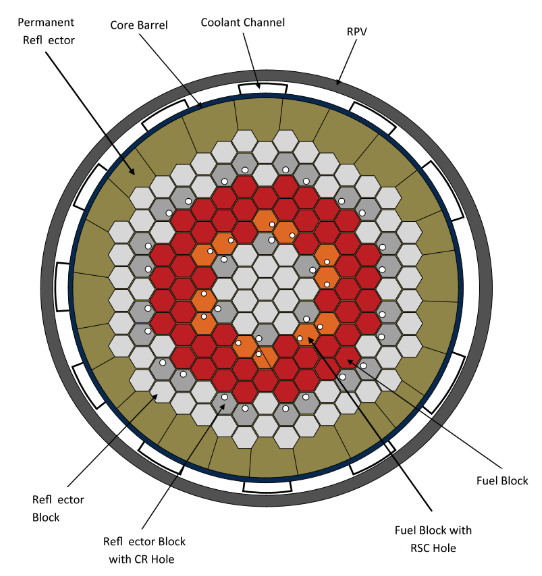
\includegraphics[width=\linewidth]{figures/radial-layout.png}
	% 		\caption{XY-plane.}
	% 	\end{subfigure}
	% 	\begin{subfigure}[t]{0.4\textwidth}
	% 		\centering
	% 		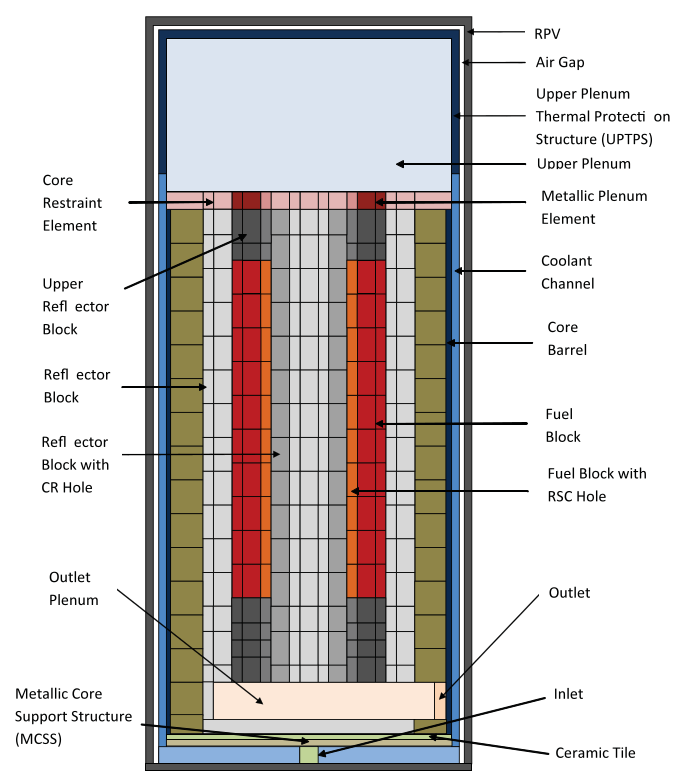
\includegraphics[width=\linewidth]{figures/axial-layout.png}
	% 		\caption{YZ-plane.}
	% 	\end{subfigure}
	% 	\hfill
	% 	\caption{MHTGR reactor layout.}
	% 	\label{fig:layout}
	% \end{figure}

	% \begin{figure}[htbp!]
	% 	\centering
	% 	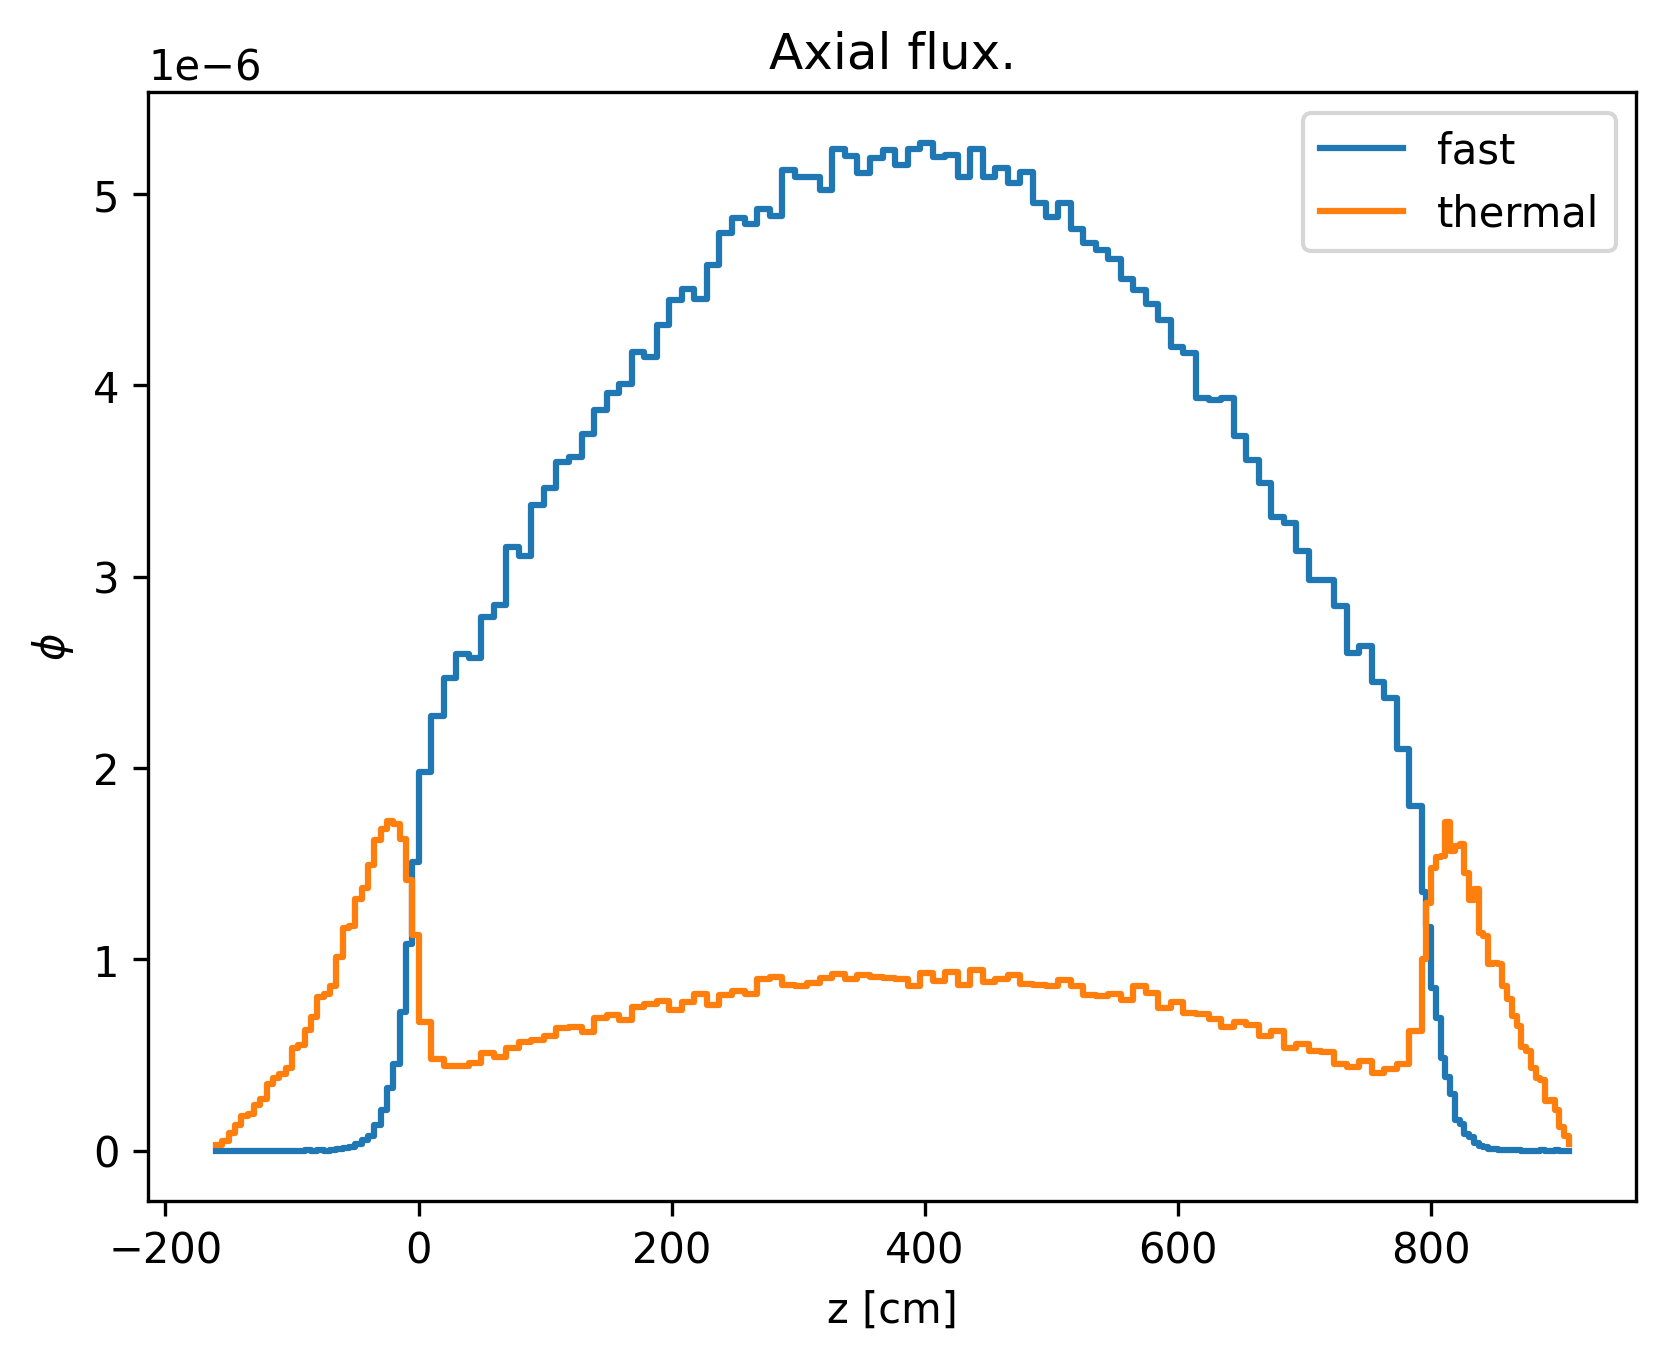
\includegraphics[width=0.6\linewidth]{figures/axial1.png}
	% 	\hfill
	% 	\caption{Neutron flux on the specified fuel channel.}
	% 	\label{fig:axial}
	% \end{figure}
